\chapter{Informationsbeschaffung}
\label{chap:Informationsbeschaffung}
Dieses Kapitel bietet fundamentale physikalische Gegebenheiten, sowie die relevanten Informationen über \ac{PIR} und verwendete 


\subsection*{Physikalische Grössen und Symbole}


\begin{table}[H]
	\begin{tabular}{l|c|c}
		
		\rowcolor{gray} Grösse &  Bezeichnung  & Einheit \\
		\hline 
		Wärmestrom &  $\dot{Q}$ & $J$  \\ 
		\rowcolor{gray}Emission & $\epsilon$ & $-$\\	
		Reflektion &  $\rho $ & $-$ \\
		\rowcolor{gray} Transmission & $\tau$ & $-$\\
		Absoprtion &  $\alpha$ & $-$  \\ 
		
		\rowcolor{gray}Geschwindigkeit des Chassis & $\dot{Q}$ & $m/s$\\
		spektrale spezifische Ausstrahlung &  $M_{\lambda }$ & $m/s^2$ \\
		\rowcolor{gray} Planksches Wirkungsquantum &  $ h$ & Js \\ 
		Lichtgeschwindigkeit im Vakuum & $c $ & $ m/s$ \\ 
		\rowcolor{gray} Stefan-Boltzmann-Konstante & $\sigma$ & $ rad/s^2 $ \\ 
	\end{tabular}
	\caption{Legende physikalische Grössen Konzeptzeichnungen}
	\label{tab:Legende Physikalische Grössen} 
\end{table} 



\section{Physikalische Aspekte}

Die Physikalischen Grundlagen erläutert auf kurze und prägnante Weise die r

\begin{table}[]
	\centering
	\label{my-label}
	\begin{tabular}{|l|l|l|}
		\hline
		\rowcolor{gray} IR-A {[}$\mu$m{]} & IR-B {[}$\mu$m{]} & IR-C {[}$\mu$m{]} \\ \hline
		0.78 - 1.4  & 1.4 - 3.0   & 3 - 1000    \\ \hline
	\end{tabular}
	\caption{Infrarotbereiche}
\end{table}

\subsection{Allgemein}

Formel für die spektrale spezifische Ausstrahlung  eines Schwarzkörpers der absoluten Temperatur  T. Für sie gilt

\begin{equation}
\label{eq5}
M_{\lambda } = \frac{2\pi h c^2 }{\lambda^5}*\frac{1}{e^\frac{hc}{\lambda k_{B}}-1}
\end{equation}
\myequations{Plank'sches Strahlungsgesetz}

Das Stefan-Boltzmann-Gesetz gibt die Strahlungsintensität Q eines idealen Temperaturstrahlers an (Integral des Plank'schen Gesetzes über alle Wellenlängen). Diese Intensität ist proportional zur 4. Potenz der absoluten Temperatur. Es lautet:
Strahlungsleistung

\begin{equation}
\label{eq1}
\frac{\mathrm{d} Q}{\mathrm{d} t} = \epsilon *\sigma * A * T^4
\end{equation}
\myequations{Wärmestrahlung}






Ein grauer Körper im Sinne der Strahlungsphysik ist ein Körper, dessen Oberfläche auftreffende Strahlung nicht vollständig absorbiert und dementsprechend auch nicht bei einer gegebenen Temperatur die maximale Strahlung (Schwarzkörperstrahlung) emittiert (siehe plancksches Strahlungsgesetz). Er hat jedoch einen wellenlängenunabhängigen Emissions- bzw. Absorptionsgrad - er erscheint „grau“, wobei sich die fehlende „Farbe“ nicht auf den sichtbaren, sondern auf den für die Messung relevanten Bereich des Spektrums bezieht.

\begin{equation}
\label{eq2}
a^2+b^2=c^2
\end{equation}
\myequations{Planksches Strahlungsgesetz}


\begin{equation}
\label{eq4}
\epsilon = \alpha  = 1
\end{equation}
\myequations{Strahlung Energieerhaltung Festkörper}

\begin{equation}
\label{eq4}
\epsilon = \varphi  = 1
\end{equation}
\myequations{Schwarzer Stahler, Energieerhaltung}



\subsection{Seebeck-Effekt}

\begin{equation}
\label{eq4}
\epsilon = \varphi  = 1
\end{equation}
\myequations{Schwarzer Stahler, Energieerhaltung}




\section{verwendete Sensorik}


\begin{figure}[H]
	\centering
	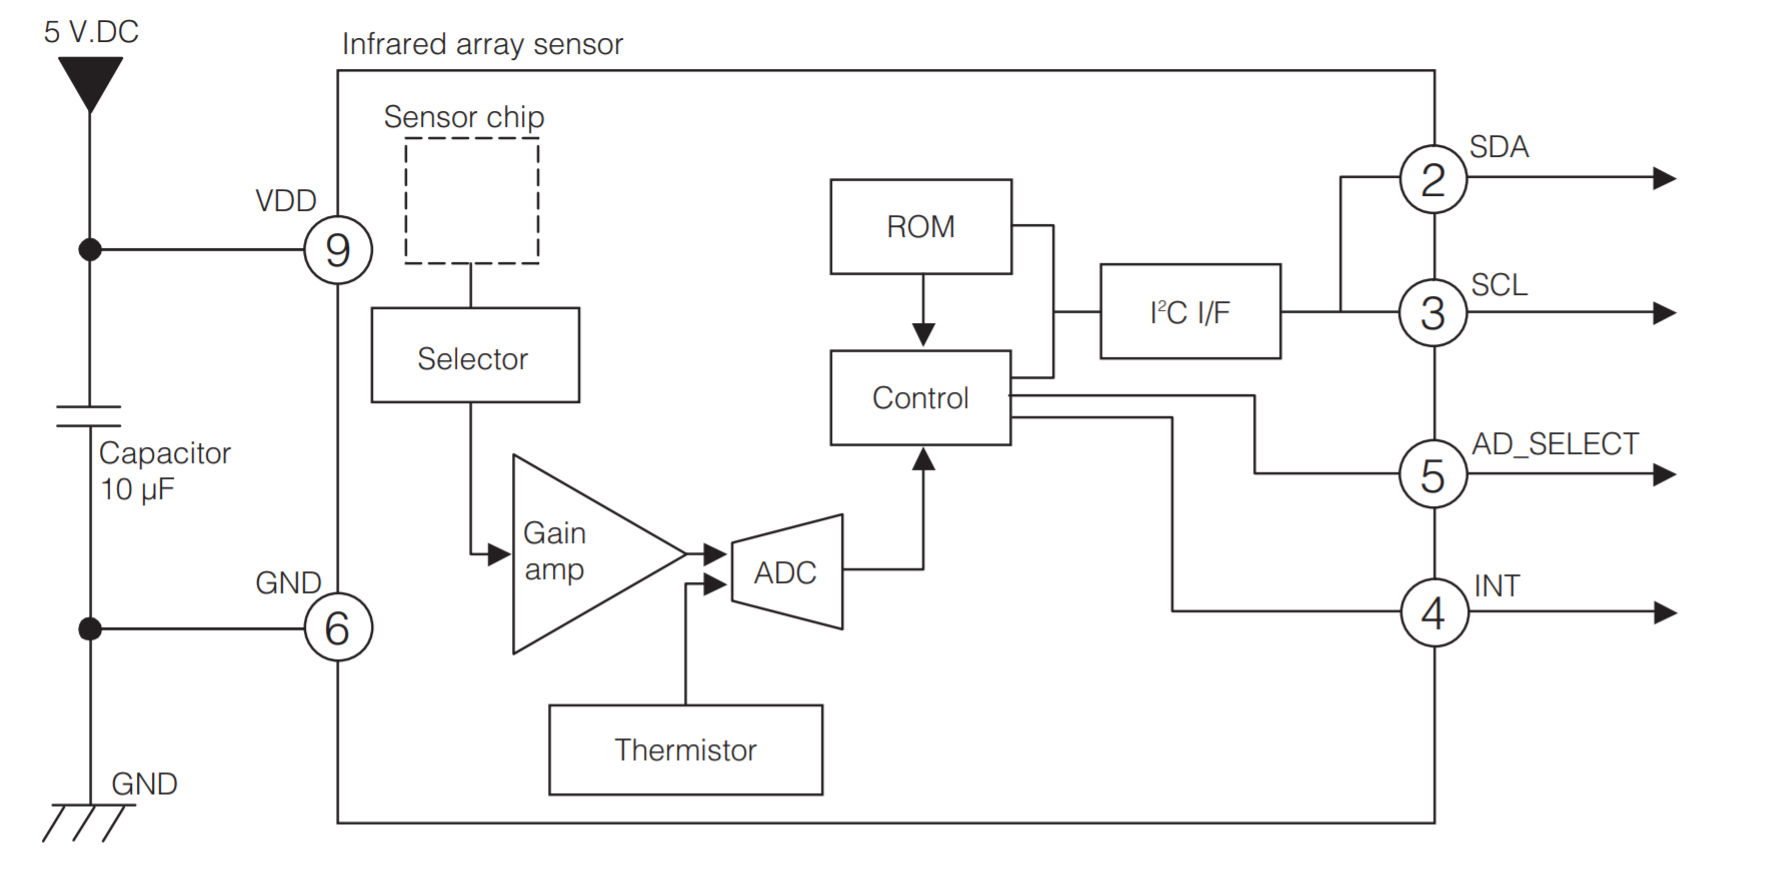
\includegraphics[width=0.8\textwidth]
	{fig/Circuit_AMG8834.PNG}
	\caption[Schema des AMG8834 Sensors]{Schema des AMG8834 Sensors} \protect\cite{AMG8834}
	\label{fig:SchemaAMG8834}
\end{figure}

Der Sensor AMG8834 ist standardmässig auf einen Emissionsgrad von $\epsilon$ =0.93 kalibriert.

\begin{figure}[H]
	\centering
	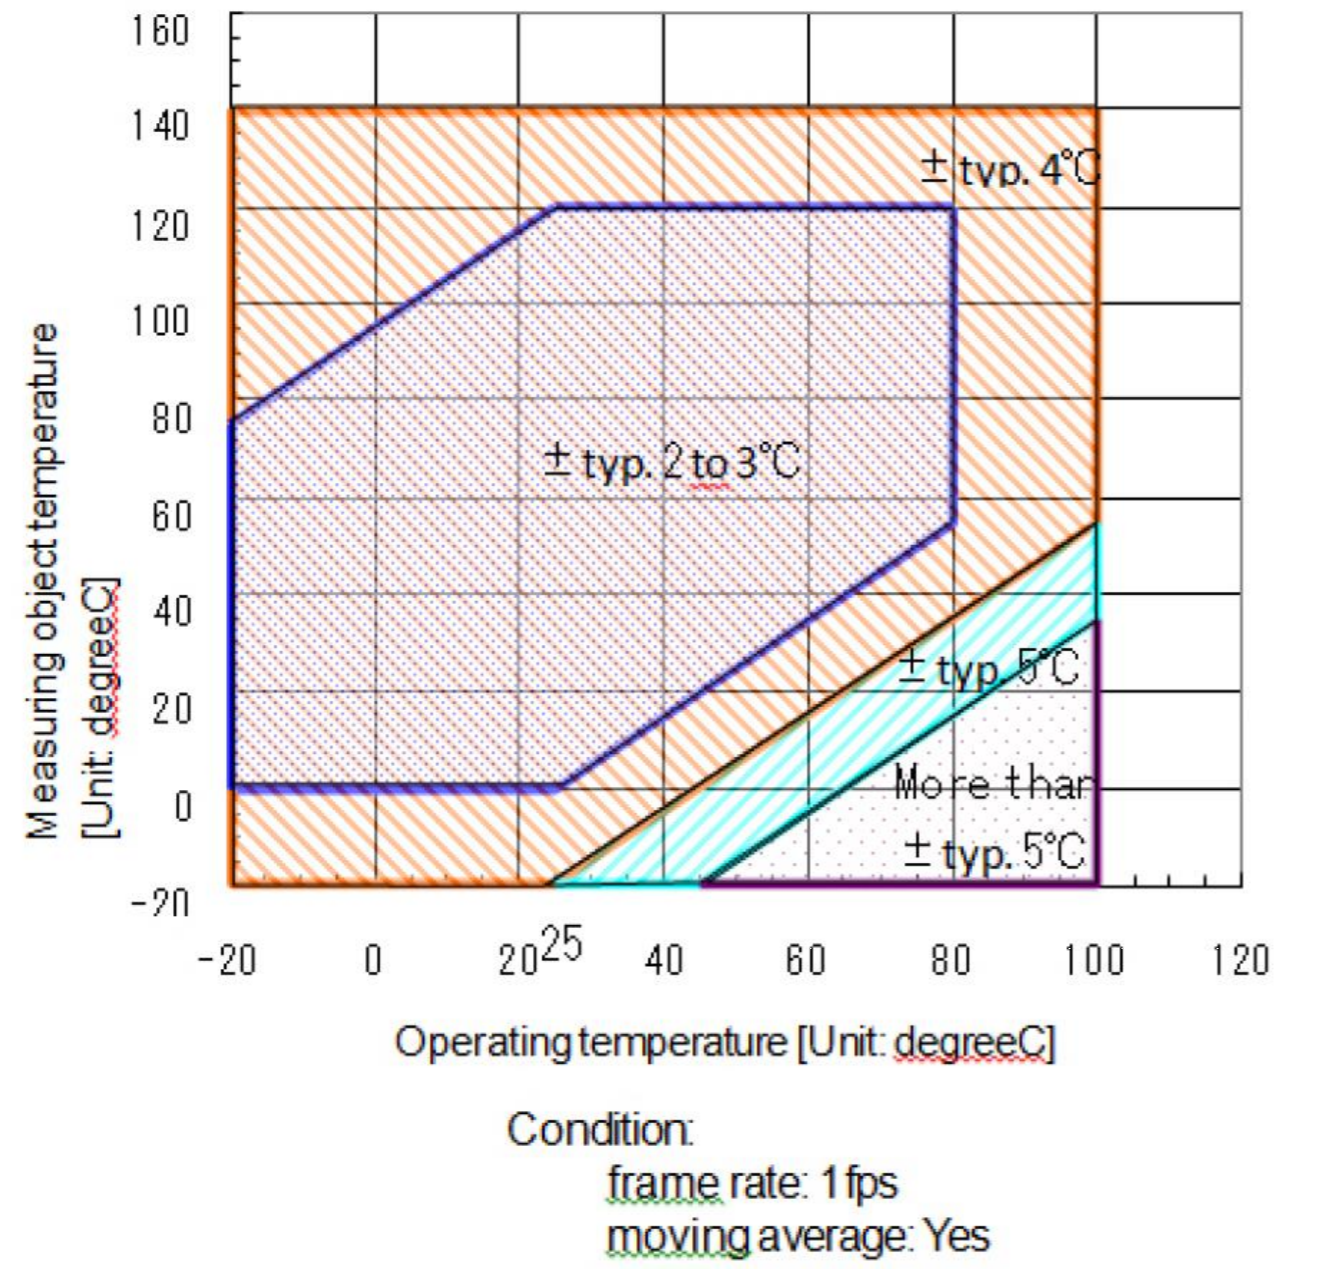
\includegraphics[width=0.8\textwidth]
	{fig/accuracy.PNG}
	\caption[Messgenauigkeit]{Messgenauigkeit} \protect\cite{AMG8834}
	\label{fig:Temperaturbereich}
\end{figure}

\begin{figure}[H]
	\centering
	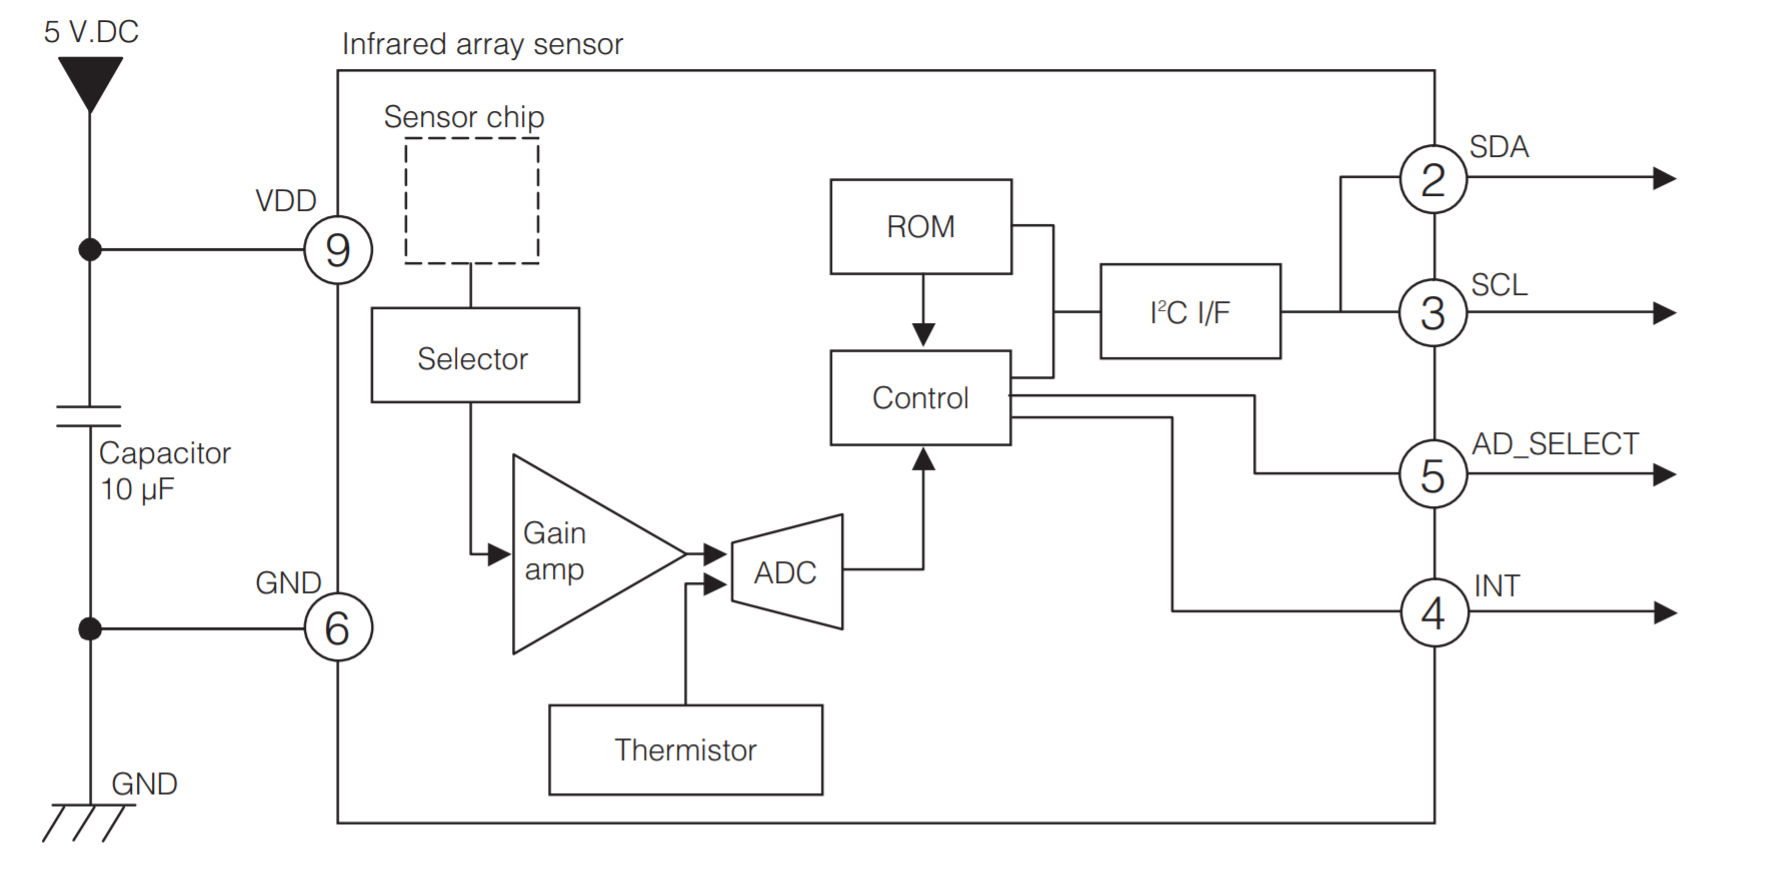
\includegraphics[width=0.8\textwidth]
	{fig/Circuit_AMG8834.PNG}
	\caption[physikalischer Aufbau AMG8834 Sensors]{physikalischer Aufbau des AMG8834 Sensors} \protect\cite{AMG8834}
	\label{fig:physAufbauAMG8834}
\end{figure}

Die eintreffenden Infrarotwellen werden durch die Silizium Linse gefiltert. Dabei fallen lediglich langwellige  Infrarotstrahlungen mit den Wellenlängen 8-13 $\mu$m. Dies entspricht dem dritten atmosphärischen Fenster.


\ac{ASIC}
\section{zu messende Objekt}

\begin{figure}[H]
	\centering
	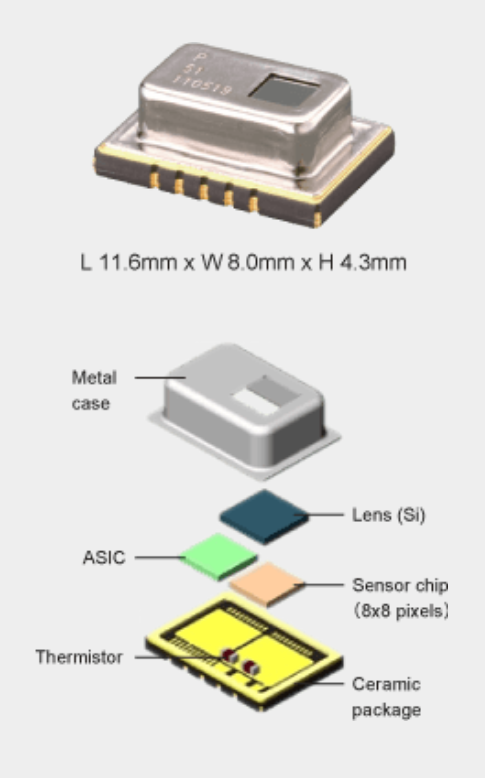
\includegraphics[width=0.5\textwidth]
	{fig/grid_eye_aufbau.PNG}
	\caption[Schema des AMG8834 Sensors]{Schema des AMG8834 Sensors} \protect\cite{AMG8834}
	\label{fig:sens}
\end{figure}
\section{geometrische Aspekte}

\section{zu messende Objekt}


\subsection{Personen}
Die Reaktionen im menschlichen Körper sind auf eine Kerntemperatur von 37 °C eingestellt
mit einer Toleranz von etwa + 0,5 Kelvin (Grad). Am wärmsten ist es in der Leber und in der
Niere, wo die intensivsten chemischen Reaktionen ablaufen, am kältesten ist die Haut, die
etwa 4 bis 7 Kelvin (Grad) kälter ist.
Die Aufteilung der verschiedenen Arten der Wärmeabgabe beträgt bei einem ruhenden
Menschen in einer Umgebung von 20 °C:

\begin{enumerate}
\item 
\begin{itemize}
	\item  46 \% Strahlung
	\item  33 \% Konvektion
	\item  19 \% Schwitzen
	\item   2 \% Atmung.
\end{itemize}
\end{enumerate}	


Die Höhe der biologisch notwendigen Wärmeabgabe hängt im wesentlichen
- von der Schwere der Tätigkeit und
- von der Größe der Körperfläche und damit von der Körpergröße des Menschen ab.


Bei einer Veränderung der oben genannten Voraussetzungen verschieben sich die Anteile.
Herrscht ein starker Wind, so erhöht sich der Anteil der Konvektion.

Diese Art der Wärmeabgabe nimmt mit der Umgebungstemperatur bis zum Wert null bei 36 °C ab. Hat die Umgebung nämlich die
Körpertemperatur erreicht, kann folglich durch Strahlung und Konvektion keine Wärme mehr
abgeführt werden.

Der schraffierte Bereich gibt die Höhe dieser Art der
Wärmeabgabe an. In einer Umgebung mit Temperaturen oberhalb 37 °C kann also die Wärme
nur noch durch Schwitzen abgeführt werden. Bei mittelschwerer Arbeit verdoppelt sich
ungefähr die Wärmeabgabe des Menschen gegenüber dem ruhigen Sitzen, da die Muskeln,
wie bereits erwähnt, zu 80 % Abwärme erzeugen. Bei schwerer Arbeit kann die Wärmeabgabe
auf ca. 300 W ansteigen. Trainierte Sportler können noch höhere Leistungen erzeugen

Die
Wärmeabgabe des Menschen ist also proportional seiner Oberfläche und damit von der Körpergröße abhängig. Die Oberfläche eines normalen Menschen beträgt ungefähr 2 m2.

Ein nackter Mensch hat beispielsweise einen k-Wert von
ungefähr 10 W/(m2·K). Damit ergibt sich aus der obigen Gleichung der Wärmestrom von 120
W für eine Umgebungstemperatur von 26 °C. \cite{MenschWaerme}

\subsection{Personenaufzüge}

In diesem Unterkapitel wurde das Messobjekt "Personenaufzug" näher betrachtet. Neben räumlichen Parametern wie Höhe, Grundfläche und Volumen spielen vor allem die Oberflächenbeschaffenheit bzw. das Oberflächenmaterial eine wichtige Rolle. Weitere thermische Einflussfaktoren finden sich in der Umgebungstemperatur un der verwendeten Leuchtmittel


\begin{figure}[H]
	\centering
	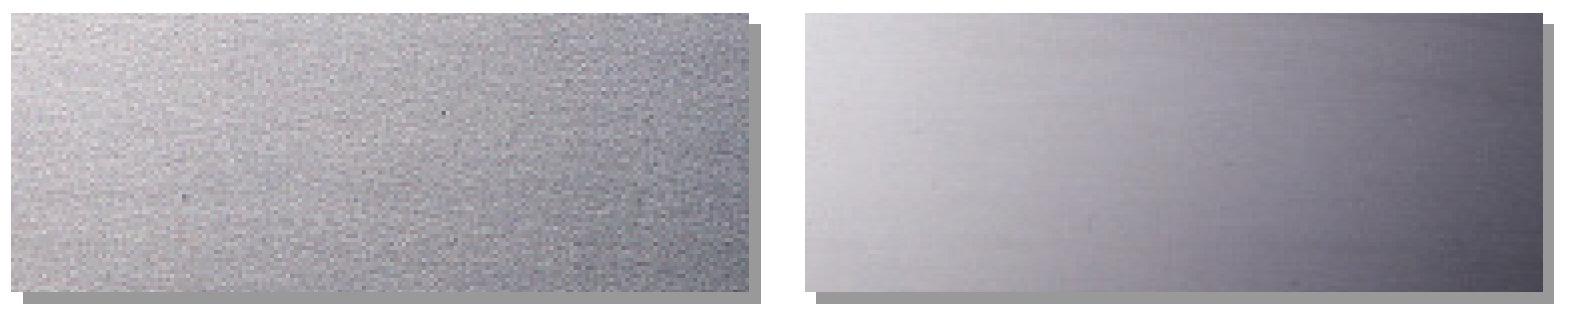
\includegraphics[width=0.8\textwidth]
	{fig/Edelstahl_gewalzt.PNG}
	\caption[Schema des AMG8834 Sensors]{Schema des AMG8834 Sensors} \protect\cite{Edelstahl}
	\label{fig:Edelstahl}
\end{figure}


\begin{figure}[H]
	\centering
	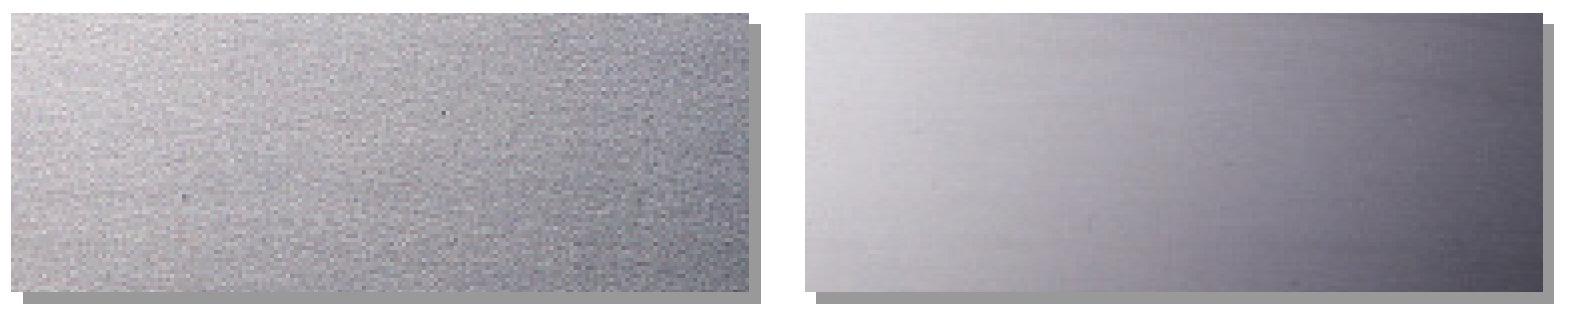
\includegraphics[width=0.8\textwidth]
	{fig/Edelstahl_gewalzt.PNG}
	\caption[Schema des AMG8834 Sensors]{Schema des AMG8834 Sensors} \protect\cite{Edelstahl}
	\label{fig:Edelstahl}
\end{figure}

\section{Störquellen}


\section{verwendete Software}